\documentclass[12pt,a4paper]{report}

\usepackage[utf8]{inputenc}
\usepackage[T1]{fontenc}
\usepackage[polish]{babel}
\usepackage{lmodern}
\usepackage{geometry}
\geometry{left=2.5cm, right=2.5cm, top=2.5cm, bottom=2.5cm}
\setlength{\headheight}{14pt}

\usepackage{amsmath,amssymb}

\usepackage{graphicx}
\usepackage{xcolor}
\usepackage{booktabs}
\usepackage{array}
\usepackage{longtable}
\usepackage{hyperref}
\usepackage{fancyhdr}
\usepackage{titlesec}
\usepackage{listings}
\usepackage{tikz}
\usepackage{tcolorbox}
\usepackage{enumitem}
\usepackage{float}
\usepackage{caption}

\usetikzlibrary{positioning, arrows.meta, shapes.geometric, calc}

\definecolor{primary}{RGB}{49, 46, 129}
\definecolor{accent}{RGB}{22, 163, 74}
\definecolor{codebg}{RGB}{248, 250, 252}
\definecolor{codeframe}{RGB}{203, 213, 225}

\hypersetup{
    colorlinks=true,
    linkcolor=primary,
    urlcolor=primary,
    citecolor=primary
}

\pagestyle{fancy}
\fancyhf{}
\fancyhead[L]{\small\textit{System Rozliczania Wydatk\'ow}}
\fancyhead[R]{\small\textit{Aplikacje Internetowe}}
\fancyfoot[C]{\thepage}
\renewcommand{\headrulewidth}{0.4pt}

\titleformat{\chapter}[display]
  {\normalfont\huge\bfseries\color{primary}}
  {\chaptertitlename\ \thechapter}{12pt}{\Huge}

\lstdefinestyle{sqlstyle}{
    language=SQL,
    backgroundcolor=\color{codebg},
    basicstyle=\ttfamily\small,
    keywordstyle=\color{primary}\bfseries,
    commentstyle=\color{gray},
    stringstyle=\color{accent},
    frame=single,
    rulecolor=\color{codeframe},
    breaklines=true,
    showstringspaces=false,
    numbers=left,
    numberstyle=\tiny\color{gray},
    captionpos=b
}

\lstdefinestyle{pseudostyle}{
    backgroundcolor=\color{codebg},
    basicstyle=\ttfamily\small,
    frame=single,
    rulecolor=\color{codeframe},
    breaklines=true,
    numbers=left,
    numberstyle=\tiny\color{gray},
    captionpos=b
}

\lstdefinestyle{envstyle}{
    backgroundcolor=\color{codebg},
    basicstyle=\ttfamily\small,
    frame=single,
    rulecolor=\color{codeframe},
    breaklines=true,
    captionpos=b
}

\newtcolorbox{infobox}[1]{
    colback=primary!5,
    colframe=primary,
    fonttitle=\bfseries,
    title=#1,
    arc=3pt
}

% --- Dane projektu (edytuj przed oddaniem) ---
\newcommand{\autor}{Krystian Oliwka}
\newcommand{\przedmiot}{Aplikacje Internetowe}
\newcommand{\kierunek}{Informatyka}
\newcommand{\rok}{2025/2026}
\newcommand{\prowadzacy}{dr hab. [Imi\k{e} Nazwisko]}

\begin{document}

% ==================== STRONA TYTUŁOWA ====================
\begin{titlepage}
    \centering
    \vspace*{1cm}
    {\Large Uniwersytet [Nazwa Uczelni]\par}
    \vspace{0.4cm}
    {\large Wydzia\l{} [Nazwa Wydzia\l{}u]\par}
    \vspace{2.5cm}

    \rule{\linewidth}{1.2pt}\\[0.6cm]
    {\Huge\bfseries\color{primary} System do Rozliczania\\[0.2cm] Wsp\'olnych Wydatk\'ow\par}
    \rule{\linewidth}{1.2pt}\\[1.5cm]

    {\LARGE Dokumentacja projektu\par}
    \vspace{2cm}

    \begin{tabular}{rl}
        \textbf{Przedmiot:}      & \przedmiot \\
        \textbf{Autor:}          & \autor \\
        \textbf{Kierunek / rok:} & \kierunek\ / \rok \\
        \textbf{Prowadz\k{a}cy:} & \prowadzacy \\
    \end{tabular}

    \vfill
    {\large \today\par}
\end{titlepage}

\pagenumbering{roman}
\tableofcontents
\clearpage
\pagenumbering{arabic}

% ==================== 1. OPIS PROJEKTU ====================
\chapter{Opis projektu}

\section{Specyfikacja tematu}

Zaprojektowano i zaimplementowano system webowy do sprawiedliwego rozliczania wsp\'olnych wydatk\'ow w grupach (np.\ wycieczki, wsp\'olne mieszkanie, imprezy). System rozwi\k{a}zuje problem nieczytelno\'sci arkuszy kalkulacyjnych przy du\.zej liczbie uczestnik\'ow i transakcji.

\begin{infobox}{G\l\'owne funkcjonalno\'sci}
\begin{itemize}[leftmargin=*]
    \item tworzenie grup rozliczeniowych i zapraszanie cz\l{}onk\'ow,
    \item dodawanie rachunk\'ow z wyborem p\l{}atnika spo\'sr\'od uczestnik\'ow,
    \item automatyczny podzia\l{} koszt\'ow na uczestnik\'ow (\texttt{bill\_splits}),
    \item rozbijanie rachunku na pozycje z paragonu (\texttt{bill\_items}) z przypisaniem do os\'ob,
    \item automatyczne bilansowanie nale\.zno\'sci (kto komu ile jest winien),
    \item system r\'ol u\.zytkownik\'ow (\texttt{user} / \texttt{admin}),
    \item triggery bazodanowe wspieraj\k{a}ce logik\k{e} systemu.
\end{itemize}
\end{infobox}

\section{Technologie}

\begin{table}[H]
\centering
\caption{Stack technologiczny}
\begin{tabular}{@{}ll@{}}
\toprule
\textbf{Warstwa} & \textbf{Technologia} \\
\midrule
J\k{e}zyk / framework & PHP 8.2, Laravel 12 \\
Baza danych & MySQL / MariaDB (produkcja), SQLite (dev) \\
Frontend & Blade, Tailwind CSS, Vite \\
Autentykacja & Laravel Breeze \\
\bottomrule
\end{tabular}
\end{table}

% ==================== 2. POZIOMY WYMAGAŃ ====================
\chapter{Poziomy wymaga\'n funkcjonalnych}

\section{Ocena 3.0 --- podstawowy CRUD i administrator}

System realizuje operacje CRUD na zasobach aplikacji. Administrator zarz\k{a}dza zasobami systemowymi.

\begin{table}[H]
\centering
\caption{Mapa operacji CRUD --- ocena 3.0}
\begin{tabular}{@{}lcccc@{}}
\toprule
\textbf{Zas\'ob} & \textbf{C} & \textbf{R} & \textbf{U} & \textbf{D} \\
\midrule
Grupy rozliczeniowe & \checkmark & \checkmark & \checkmark & \checkmark \\
Rachunki / wydatki   & \checkmark & \checkmark & ---        & \checkmark \\
U\.zytkownicy (panel admina) & --- & \checkmark & \checkmark & \checkmark \\
\bottomrule
\end{tabular}
\end{table}

Administrator (\texttt{role = admin}) zarz\k{a}dza u\.zytkownikami w panelu \texttt{/admin/users}.

\section{Ocena 4.0 --- rozszerzone uprawnienia}

\begin{itemize}[leftmargin=*]
    \item kolumna \texttt{users.role} przyjmuje warto\'sci \texttt{user} lub \texttt{admin},
    \item zwyk\l{}y u\.zytkownik zarz\k{a}dza w\l{}asnymi grupami (tworzenie, edycja, usuwanie, dodawanie cz\l{}onk\'ow),
    \item administrator widzi wszystkie grupy, mo\.ze je edytowa\'c i usuwa\'c,
    \item administrator zarz\k{a}dza profilami i rolami innych u\.zytkownik\'ow,
    \item kontrola dost\k{e}pu realizowana przez \texttt{AdminMiddleware}.
\end{itemize}

\section{Ocena 5.0 --- zaawansowana logika biznesowa}

\begin{itemize}[leftmargin=*]
    \item \textbf{Wielu p\l{}atnik\'ow} --- przy dodawaniu rachunku wybiera si\k{e} p\l{}atnika z listy cz\l{}onk\'ow grupy.
    \item \textbf{Podzia\l{} koszt\'ow} --- tabela \texttt{bill\_splits}; przy dodaniu rachunku tworzone s\k{a} rekordy z r\'ownym udzia\l{}em.
    \item \textbf{Pozycje z paragonu} --- tabele \texttt{bill\_items} i \texttt{bill\_item\_user}.
    \item \textbf{Bilansowanie} --- algorytm: saldo = zap\l{}acone $-$ nale\.zno\'sci; na MySQL wspierane funkcj\k{a} sk\l{}adow\k{a}.
    \item \textbf{Triggery DB} --- automatyczna aktualizacja \texttt{groups.total\_amount} oraz walidacja cz\l{}onkostwa w grupie.
\end{itemize}

% ==================== 3. BAZA DANYCH ====================
\chapter{Aspekt projektowy bazy danych}

\section{Diagram ERD}

\begin{figure}[H]
\centering
\begin{tikzpicture}[
    entity/.style={draw=primary, thick, rounded corners=4pt, minimum width=2.8cm, minimum height=1.1cm, align=center, fill=primary!8, font=\small\bfseries},
    rel/.style={-{Stealth[length=2.5mm]}, thick, primary},
    label/.style={font=\scriptsize, fill=white, inner sep=1pt}
]

\node[entity] (users) {users};
\node[entity, below left=2.2cm and 0.5cm of users] (groups) {groups};
\node[entity, below right=2.2cm and 0.5cm of users] (gu) {group\_user};
\node[entity, below=2cm of groups] (bills) {bills};
\node[entity, below left=1.8cm and 0.3cm of bills] (items) {bill\_items};
\node[entity, below right=1.8cm and 0.3cm of bills] (splits) {bill\_splits};
\node[entity, below=1.6cm of items] (biu) {bill\_item\_user};

\draw[rel] (users) -- node[label, above left] {owner\_id} (groups);
\draw[rel] (users) -- (gu);
\draw[rel] (groups) -- (gu);
\draw[rel] (groups) -- node[label, right] {1:N} (bills);
\draw[rel] (users) -- node[label, above] {payer\_id} (bills);
\draw[rel] (bills) -- (items);
\draw[rel] (bills) -- (splits);
\draw[rel] (users) -- (splits);
\draw[rel] (items) -- (biu);
\draw[rel] (users) -- (biu);

\end{tikzpicture}
\caption{Diagram encji i powi\k{a}za\'n (ERD)}
\end{figure}

\section{Opis struktur tabel}

\begin{longtable}{@{}p{3.2cm}p{10.5cm}@{}}
\toprule
\textbf{Tabela} & \textbf{Opis i kluczowe kolumny} \\
\midrule
\endhead
\texttt{users} &
Konta u\.zytkownik\'ow. Kolumny: \texttt{id}, \texttt{name}, \texttt{email}, \texttt{password}, \texttt{role} (\texttt{user}/\texttt{admin}). \\
\texttt{groups} &
Grupy rozliczeniowe. \texttt{owner\_id} $\rightarrow$ \texttt{users.id}. \texttt{total\_amount} utrzymywane przez trigger. \\
\texttt{group\_user} &
Tabela \l{}\k{a}cznikowa M:N --- cz\l{}onkostwo w grupie. \\
\texttt{bills} &
Rachunki grupowe. \texttt{payer\_id} wskazuje p\l{}atnika. \texttt{amount}, \texttt{description}, \texttt{date}. \\
\texttt{bill\_splits} &
Udzia\l{} ka\.zdego u\.zytkownika w danym rachunku. \texttt{is\_paid} --- czy sp\l{}acone. \\
\texttt{bill\_items} &
Pozycje z paragonu (np.\ Pizza, Nap\'oj). \texttt{price}, \texttt{quantity}. \\
\texttt{bill\_item\_user} &
Przypisanie pozycji paragonu do u\.zytkownik\'ow (M:N). \\
\bottomrule
\caption{Opis tabel bazy danych}
\end{longtable}

\section{Kod SQL tworz\k{a}cy baz\k{e}}

\begin{lstlisting}[style=sqlstyle, caption={Tabela u\.zytkownik\'ow}]
CREATE TABLE users (
    id BIGINT UNSIGNED AUTO_INCREMENT PRIMARY KEY,
    name VARCHAR(255) NOT NULL,
    email VARCHAR(255) NOT NULL UNIQUE,
    role VARCHAR(255) NOT NULL DEFAULT 'user',
    password VARCHAR(255) NOT NULL,
    email_verified_at TIMESTAMP NULL,
    remember_token VARCHAR(100) NULL,
    created_at TIMESTAMP NULL,
    updated_at TIMESTAMP NULL
);
\end{lstlisting}

\begin{lstlisting}[style=sqlstyle, caption={Grupy rozliczeniowe}]
CREATE TABLE groups (
    id BIGINT UNSIGNED AUTO_INCREMENT PRIMARY KEY,
    name VARCHAR(255) NOT NULL,
    owner_id BIGINT UNSIGNED NOT NULL,
    total_amount DECIMAL(12,2) DEFAULT 0.00,
    created_at TIMESTAMP NULL,
    updated_at TIMESTAMP NULL,
    FOREIGN KEY (owner_id) REFERENCES users(id) ON DELETE CASCADE
);
\end{lstlisting}

\begin{lstlisting}[style=sqlstyle, caption={Rachunki}]
CREATE TABLE bills (
    id BIGINT UNSIGNED AUTO_INCREMENT PRIMARY KEY,
    group_id BIGINT UNSIGNED NOT NULL,
    payer_id BIGINT UNSIGNED NOT NULL,
    description VARCHAR(255) NOT NULL,
    amount DECIMAL(10,2) NOT NULL,
    date DATE NOT NULL,
    created_at TIMESTAMP NULL,
    updated_at TIMESTAMP NULL,
    FOREIGN KEY (group_id) REFERENCES groups(id) ON DELETE CASCADE,
    FOREIGN KEY (payer_id) REFERENCES users(id) ON DELETE CASCADE
);
\end{lstlisting}

\begin{lstlisting}[style=sqlstyle, caption={Podzia\l{} koszt\'ow i pozycje paragonu}]
CREATE TABLE bill_splits (
    id BIGINT UNSIGNED AUTO_INCREMENT PRIMARY KEY,
    bill_id BIGINT UNSIGNED NOT NULL,
    user_id BIGINT UNSIGNED NOT NULL,
    amount DECIMAL(10,2) NOT NULL,
    is_paid BOOLEAN DEFAULT FALSE,
    created_at TIMESTAMP NULL,
    updated_at TIMESTAMP NULL,
    FOREIGN KEY (bill_id) REFERENCES bills(id) ON DELETE CASCADE,
    FOREIGN KEY (user_id) REFERENCES users(id) ON DELETE CASCADE
);

CREATE TABLE bill_items (
    id BIGINT UNSIGNED AUTO_INCREMENT PRIMARY KEY,
    bill_id BIGINT UNSIGNED NOT NULL,
    name VARCHAR(255) NOT NULL,
    price DECIMAL(10,2) NOT NULL,
    quantity INT DEFAULT 1,
    created_at TIMESTAMP NULL,
    updated_at TIMESTAMP NULL,
    FOREIGN KEY (bill_id) REFERENCES bills(id) ON DELETE CASCADE
);

CREATE TABLE bill_item_user (
    id BIGINT UNSIGNED AUTO_INCREMENT PRIMARY KEY,
    bill_item_id BIGINT UNSIGNED NOT NULL,
    user_id BIGINT UNSIGNED NOT NULL,
    FOREIGN KEY (bill_item_id) REFERENCES bill_items(id) ON DELETE CASCADE,
    FOREIGN KEY (user_id) REFERENCES users(id) ON DELETE CASCADE
);
\end{lstlisting}

% ==================== 4. TRIGGERY ====================
\chapter{Mechanizmy bazodanowe (triggery i funkcje)}

\section{Wymaganie techniczne}

Projekt implementuje \textbf{obowi\k{a}zkowe triggery bazodanowe} w dialekcie MySQL. Kod znajduje si\k{e} w migracji \texttt{2026\_05\_14\_163307\_add\_trigger\_and\_total\_to\_groups.php}.

\section{Triggery automatyzacji --- \texttt{total\_amount}}

Trzy triggery na tabeli \texttt{bills} automatycznie aktualizuj\k{a} pole \texttt{groups.total\_amount}:

\begin{lstlisting}[style=sqlstyle, caption={Trigger po INSERT na bills}]
CREATE TRIGGER update_group_total_after_bill_insert
AFTER INSERT ON bills FOR EACH ROW
BEGIN
    UPDATE groups
    SET total_amount = total_amount + NEW.amount
    WHERE id = NEW.group_id;
END;
\end{lstlisting}

\begin{lstlisting}[style=sqlstyle, caption={Trigger po UPDATE na bills}]
CREATE TRIGGER update_group_total_after_bill_update
AFTER UPDATE ON bills FOR EACH ROW
BEGIN
    UPDATE groups
    SET total_amount = total_amount - OLD.amount + NEW.amount
    WHERE id = NEW.group_id;
END;
\end{lstlisting}

\begin{lstlisting}[style=sqlstyle, caption={Trigger po DELETE na bills}]
CREATE TRIGGER update_group_total_after_bill_delete
AFTER DELETE ON bills FOR EACH ROW
BEGIN
    UPDATE groups
    SET total_amount = total_amount - OLD.amount
    WHERE id = OLD.group_id;
END;
\end{lstlisting}

\section{Trigger walidacyjny --- cz\l{}onkostwo w grupie}

Przed przypisaniem pozycji paragonu do u\.zytkownika trigger sprawdza, czy u\.zytkownik nale\.zy do grupy:

\begin{lstlisting}[style=sqlstyle, caption={Walidacja przy INSERT na bill\_item\_user}]
CREATE TRIGGER validate_user_in_group_before_item_assign
BEFORE INSERT ON bill_item_user FOR EACH ROW
BEGIN
    DECLARE v_group_id INT;
    DECLARE v_is_member INT DEFAULT 0;

    SELECT b.group_id INTO v_group_id
    FROM bill_items bi
    JOIN bills b ON bi.bill_id = b.id
    WHERE bi.id = NEW.bill_item_id;

    SELECT COUNT(*) INTO v_is_member
    FROM group_user
    WHERE group_id = v_group_id AND user_id = NEW.user_id;

    IF v_is_member = 0 THEN
        SIGNAL SQLSTATE '45000'
        SET MESSAGE_TEXT = 'Blad Walidacji DB: Uzytkownik nie nalezy do tej grupy!';
    END IF;
END;
\end{lstlisting}

\section{Funkcja sk\l{}adowa \texttt{get\_user\_net\_balance}}

\begin{lstlisting}[style=sqlstyle, caption={Obliczanie salda netto u\.zytkownika w grupie}]
CREATE FUNCTION get_user_net_balance(p_user_id INT, p_group_id INT)
RETURNS DECIMAL(10,2) DETERMINISTIC
BEGIN
    DECLARE v_total_paid DECIMAL(10,2) DEFAULT 0.00;
    DECLARE v_total_owed DECIMAL(10,2) DEFAULT 0.00;

    SELECT IFNULL(SUM(amount), 0.00) INTO v_total_paid
    FROM bills
    WHERE payer_id = p_user_id AND group_id = p_group_id;

    SELECT IFNULL(SUM(bs.amount), 0.00) INTO v_total_owed
    FROM bill_splits bs
    JOIN bills b ON bs.bill_id = b.id
    WHERE bs.user_id = p_user_id AND b.group_id = p_group_id;

    RETURN v_total_paid - v_total_owed;
END;
\end{lstlisting}

Funkcja jest wywo\l{}ywana w modelu \texttt{Group::getBalances()} przy po\l{}\k{a}czeniu z MySQL.

% ==================== 5. ALGORYTMY ====================
\chapter{Za\l{}o\.zenia funkcjonalne i algorytmy}

\section{Mechanizmy CRUD w aplikacji}

\begin{table}[H]
\centering
\caption{Mapa kontroler\'ow i tras}
\begin{tabular}{@{}lll@{}}
\toprule
\textbf{Zas\'ob} & \textbf{Kontroler} & \textbf{Trasy} \\
\midrule
Grupy & \texttt{GroupController} & \texttt{groups.*} \\
Rachunki & \texttt{BillController} & \texttt{bills.store}, \texttt{bills.destroy} \\
Pozycje paragonu & \texttt{BillItemController} & \texttt{bill-items.store} \\
U\.zytkownicy (admin) & \texttt{Admin\textbackslash UserController} & \texttt{admin.users.*} \\
Profil & \texttt{ProfileController} & \texttt{profile.*} \\
\bottomrule
\end{tabular}
\end{table}

\section{Algorytm 1: R\'owny podzia\l{} rachunku}

\begin{lstlisting}[style=pseudostyle, caption={Pseudokod --- tworzenie bill\_splits}]
WEJSCIE: rachunek R o kwocie K, grupa G z N czlonkami
WYJSCIE: rekordy w tabeli bill_splits

udzial = K / N
DLA KAZDEGO czlonka C z grupy G:
    UTWORZ bill_split(bill_id=R, user_id=C, amount=udzial)
    JESLI C jest platnikiem:
        ustaw is_paid = TRUE
\end{lstlisting}

Implementacja: \texttt{BillController::createEqualSplits()}.

\section{Algorytm 2: Bilans u\.zytkownika w grupie}

\begin{lstlisting}[style=pseudostyle, caption={Pseudokod --- obliczanie salda}]
WEJSCIE: user_id U, group_id G
WYJSCIE: saldo S

zaplacone = SUMA(bills.amount WHERE payer_id=U AND group_id=G)
naleznosci = SUMA(bill_splits.amount WHERE user_id=U AND bill IN G)
S = zaplacone - naleznosci

JESLI S > 0:  inni winni U kwote S
JESLI S < 0:  U winien innym kwote |S|
JESLI S = 0:  rozliczony
\end{lstlisting}

Implementacja: \texttt{Group::getBalances()} oraz funkcja SQL \texttt{get\_user\_net\_balance()}.

\section{Przyk\l{}ad dzia\l{}ania}

Grupa 3-osobowa. Krystian p\l{}aci 600\,z\l{} za obiad. Ka\.zdy dostaje udzia\l{} 200\,z\l{}:

\begin{table}[H]
\centering
\begin{tabular}{@{}lrr@{}}
\toprule
\textbf{Osoba} & \textbf{Zap\l{}aci\l{}a} & \textbf{Saldo} \\
\midrule
Krystian & 600\,z\l{} & $+400$\,z\l{} \\
Adam     & 0\,z\l{}   & $-200$\,z\l{} \\
Ewa      & 0\,z\l{}   & $-200$\,z\l{} \\
\bottomrule
\end{tabular}
\caption{Przyk\l{}adowe salda po rachunku 600\,z\l{}}
\end{table}

% ==================== 6. DOSTĘP ZDALNY ====================
\chapter{Koncepcja dost\k{e}pu zdalnego do bazy danych}

\section{Za\l{}o\.zenia}

\begin{itemize}[leftmargin=*]
    \item Baza MySQL/MariaDB hostowana lokalnie (XAMPP, Laragon) lub na serwerze zdalnym.
    \item Dost\k{e}p administracyjny przez phpMyAdmin, HeidiSQL lub MySQL Workbench.
    \item Aplikacja \l{}\k{a}czy si\k{e} z baz\k{a} przez PDO --- konfiguracja w pliku \texttt{.env}.
\end{itemize}

\section{Konfiguracja po\l{}\k{a}czenia}

\begin{lstlisting}[style=envstyle, caption={Fragment pliku .env}]
DB_CONNECTION=mysql
DB_HOST=127.0.0.1
DB_PORT=3306
DB_DATABASE=rozliczenia
DB_USERNAME=root
DB_PASSWORD=
\end{lstlisting}

\section{Zrzuty ekranu z aplikacji}

Poni\.zej przedstawiono zrzuty ekranu z dzia\l{}aj\k{a}cej aplikacji webowej. Triggery i funkcja sk\l{}adowa s\k{a} zaimplementowane w kodzie SQL (rozdzia\l{} 4) --- w trybie deweloperskim projekt korzysta z SQLite (\texttt{database/database.sqlite}), na produkcji z MySQL.

\begin{figure}[H]
    \centering
    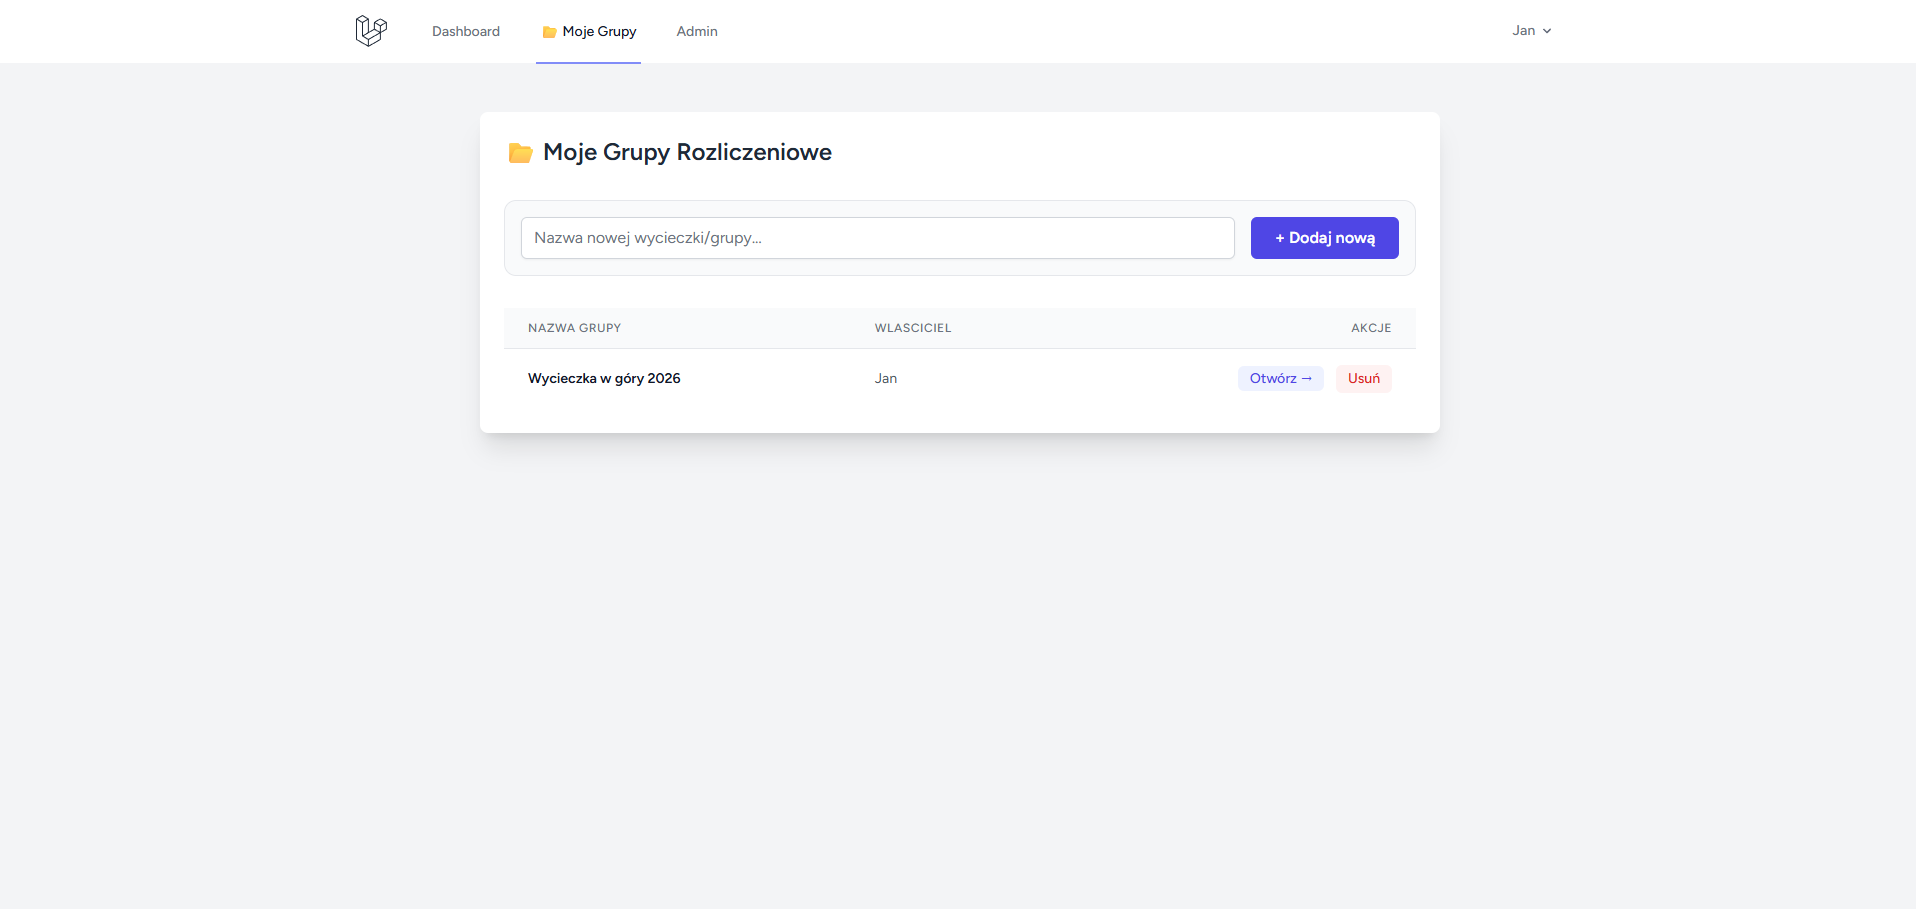
\includegraphics[width=0.92\textwidth]{screenshots/01-lista-grup.png}
    \caption{Lista grup rozliczeniowych u\.zytkownika}
\end{figure}

\begin{figure}[H]
    \centering
    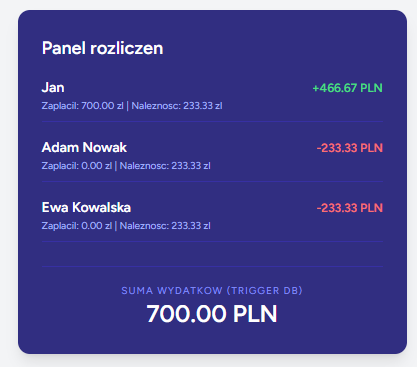
\includegraphics[width=0.92\textwidth]{screenshots/02-panel-rozliczen.png}
    \caption{Panel rozlicze\'n --- salda cz\l{}onk\'ow grupy}
\end{figure}

\begin{figure}[H]
    \centering
    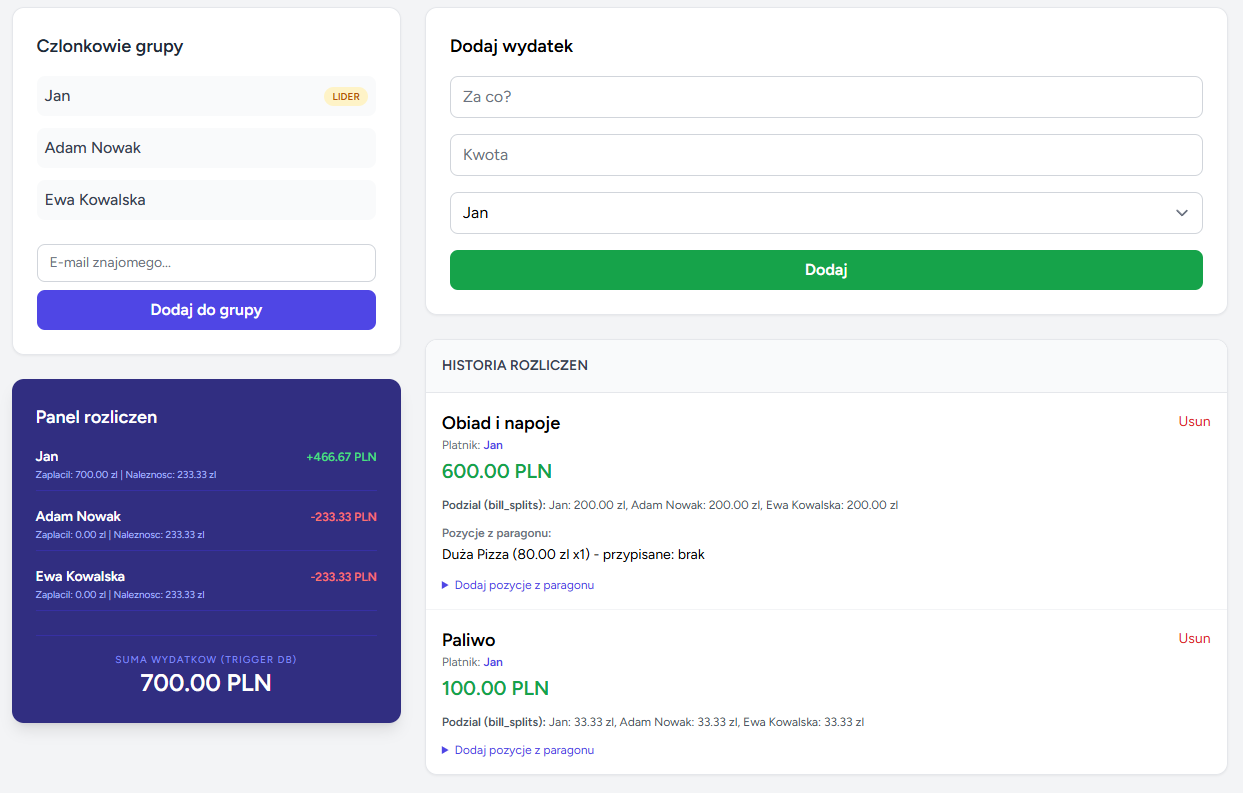
\includegraphics[width=0.92\textwidth]{screenshots/03-rachunek-i-splits.png}
    \caption{Historia rachunk\'ow z podzia\l{}em koszt\'ow (\texttt{bill\_splits}) i pozycjami paragonu}
\end{figure}

\begin{figure}[H]
    \centering
    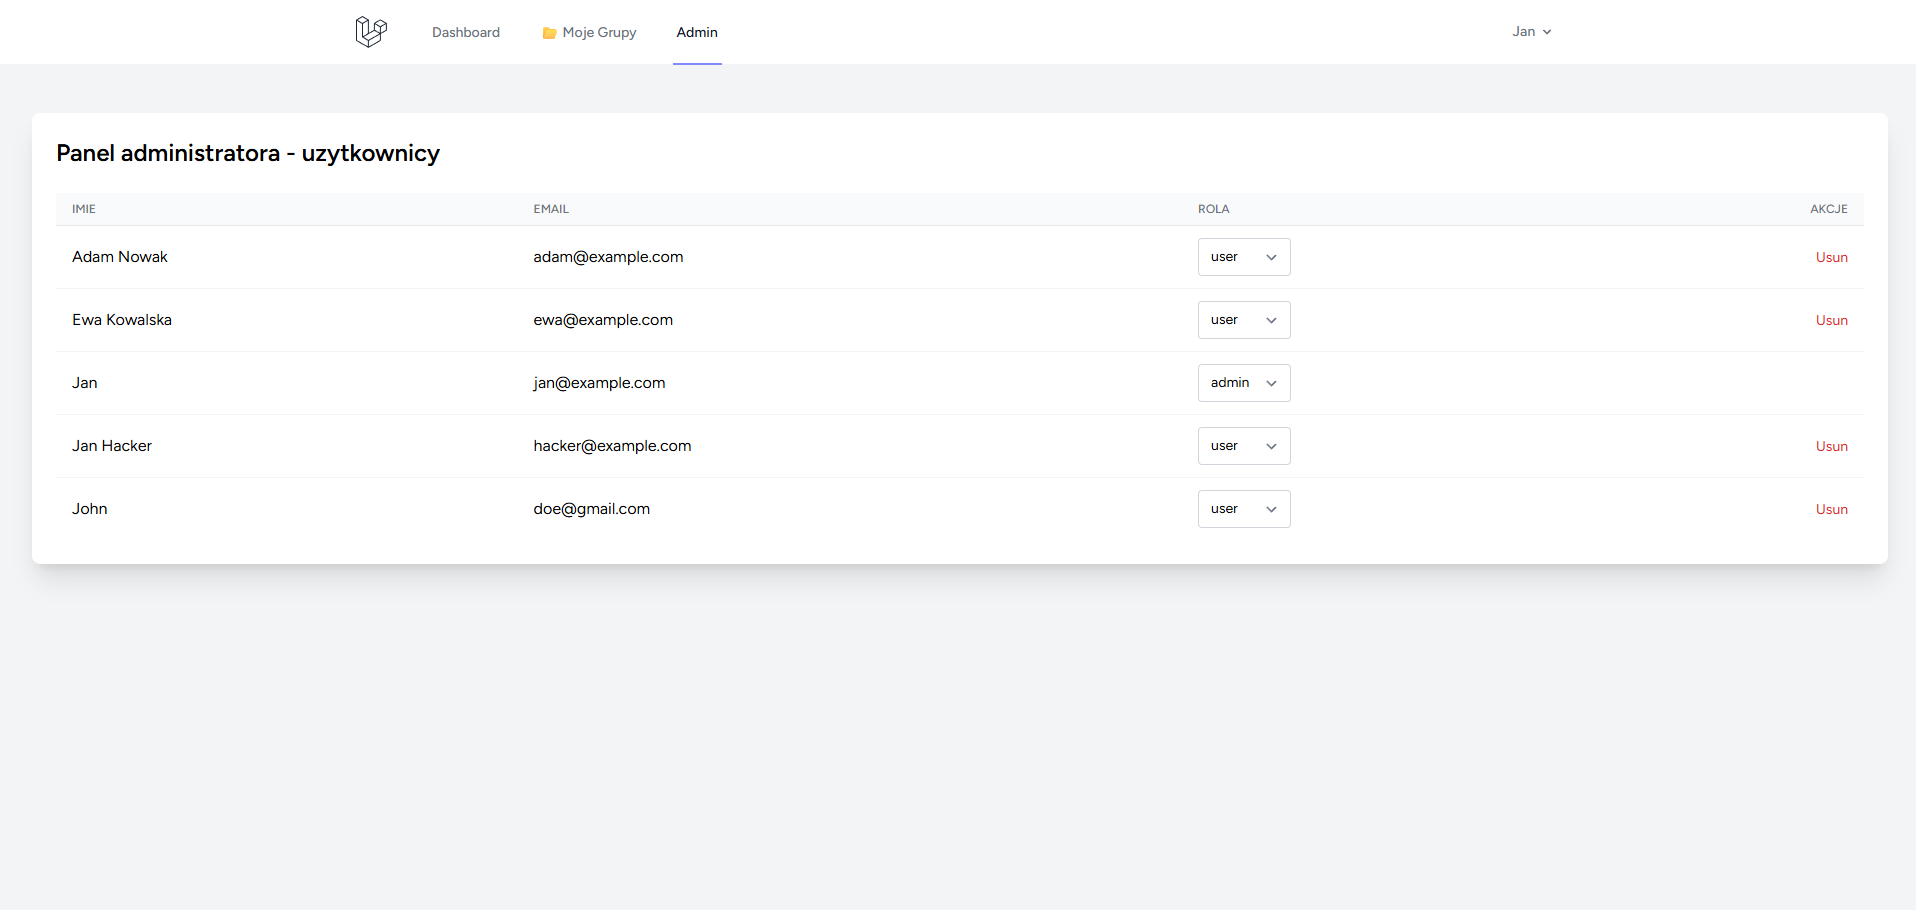
\includegraphics[width=0.92\textwidth]{screenshots/04-panel-admina.png}
    \caption{Panel administratora --- zarz\k{a}dzanie u\.zytkownikami i rolami}
\end{figure}

% ==================== 7. URUCHOMIENIE ====================
\chapter{Uruchomienie i testowanie}

\section{Wymagania \.srodowiskowe}

PHP 8.2+, Composer, Node.js. Instrukcja szczeg\'o\l{}owa w pliku \texttt{JAK\_URUCHOMIC.md}.

\section{Kroki uruchomienia}

\begin{enumerate}[leftmargin=*]
    \item \texttt{composer install} i \texttt{npm install}
    \item Skopiuj \texttt{.env.example} $\rightarrow$ \texttt{.env}, wygeneruj klucz: \texttt{php artisan key:generate}
    \item Uruchom migracje: \texttt{php artisan migrate:fresh --seed}
    \item Zbuduj frontend: \texttt{npm run build}
    \item Uruchom serwer: \texttt{php artisan serve} $\rightarrow$ \url{http://127.0.0.1:8000}
\end{enumerate}

\section{Konta testowe}

\begin{table}[H]
\centering
\begin{tabular}{@{}lll@{}}
\toprule
\textbf{Rola} & \textbf{E-mail} & \textbf{Has\l{}o} \\
\midrule
admin & \texttt{krystian@example.com} & \texttt{password} \\
user  & \texttt{adam@example.com}     & \texttt{password} \\
user  & \texttt{ewa@example.com}      & \texttt{password} \\
\bottomrule
\end{tabular}
\caption{Konta demonstracyjne po seedzie}
\end{table}

\section{Scenariusz testowy}

\begin{enumerate}[leftmargin=*]
    \item Zaloguj si\k{e} jako administrator (\texttt{krystian@example.com}).
    \item Przejd\'z do \emph{Moje Grupy} $\rightarrow$ otw\'orz \emph{Wycieczka w g\'ory 2026}.
    \item Sprawd\'z panel rozlicze\'n --- salda cz\l{}onk\'ow.
    \item Dodaj nowy wydatek z wybranym p\l{}atnikiem.
    \item Dodaj pozycj\k{e} z paragonu i przypisz j\k{a} do os\'ob.
    \item Wejd\'z w panel \emph{Admin} --- zmie\'n rol\k{e} u\.zytkownika.
    \item Wyloguj si\k{e}, zaloguj jako \texttt{adam@example.com} --- sprawd\'z widoczno\'s\'c grupy.
\end{enumerate}

% ==================== 8. STRUKTURA ====================
\chapter{Struktura projektu}

\begin{lstlisting}[style=pseudostyle, caption={Struktura repozytorium}]
AplikacjeInternetoweProjekt/
  Dokumentacja/
    dokumentacja.pdf      -- dokumentacja do oddania
    dokumentacja.tex      -- zrodlo LaTeX
    screenshots/          -- zrzuty ekranu
  ProjektAplikacje/       -- aplikacja Laravel
    app/Http/Controllers/
    app/Http/Middleware/
    app/Models/
    database/migrations/
    database/seeders/
    resources/views/
    routes/web.php
\end{lstlisting}

\appendix
\chapter{Spis plik\'ow migracji}

\begin{table}[H]
\centering
\small
\begin{tabular}{@{}p{7cm}p{6cm}@{}}
\toprule
\textbf{Plik migracji} & \textbf{Zawarto\'s\'c} \\
\midrule
\texttt{create\_users\_table} & Tabela u\.zytkownik\'ow \\
\texttt{add\_role\_to\_users\_table} & Kolumna \texttt{role} \\
\texttt{create\_groups\_table} & Grupy + \texttt{total\_amount} \\
\texttt{create\_group\_user\_table} & Cz\l{}onkostwo M:N \\
\texttt{create\_bills\_table} & Rachunki \\
\texttt{create\_bill\_items\_table} & Pozycje + \texttt{bill\_item\_user} \\
\texttt{create\_bill\_splits\_table} & Podzia\l{} koszt\'ow \\
\texttt{add\_trigger\_and\_total\_to\_groups} & Triggery + funkcja SQL \\
\bottomrule
\end{tabular}
\end{table}

\end{document}
